\begin{figure}[t]
\centering
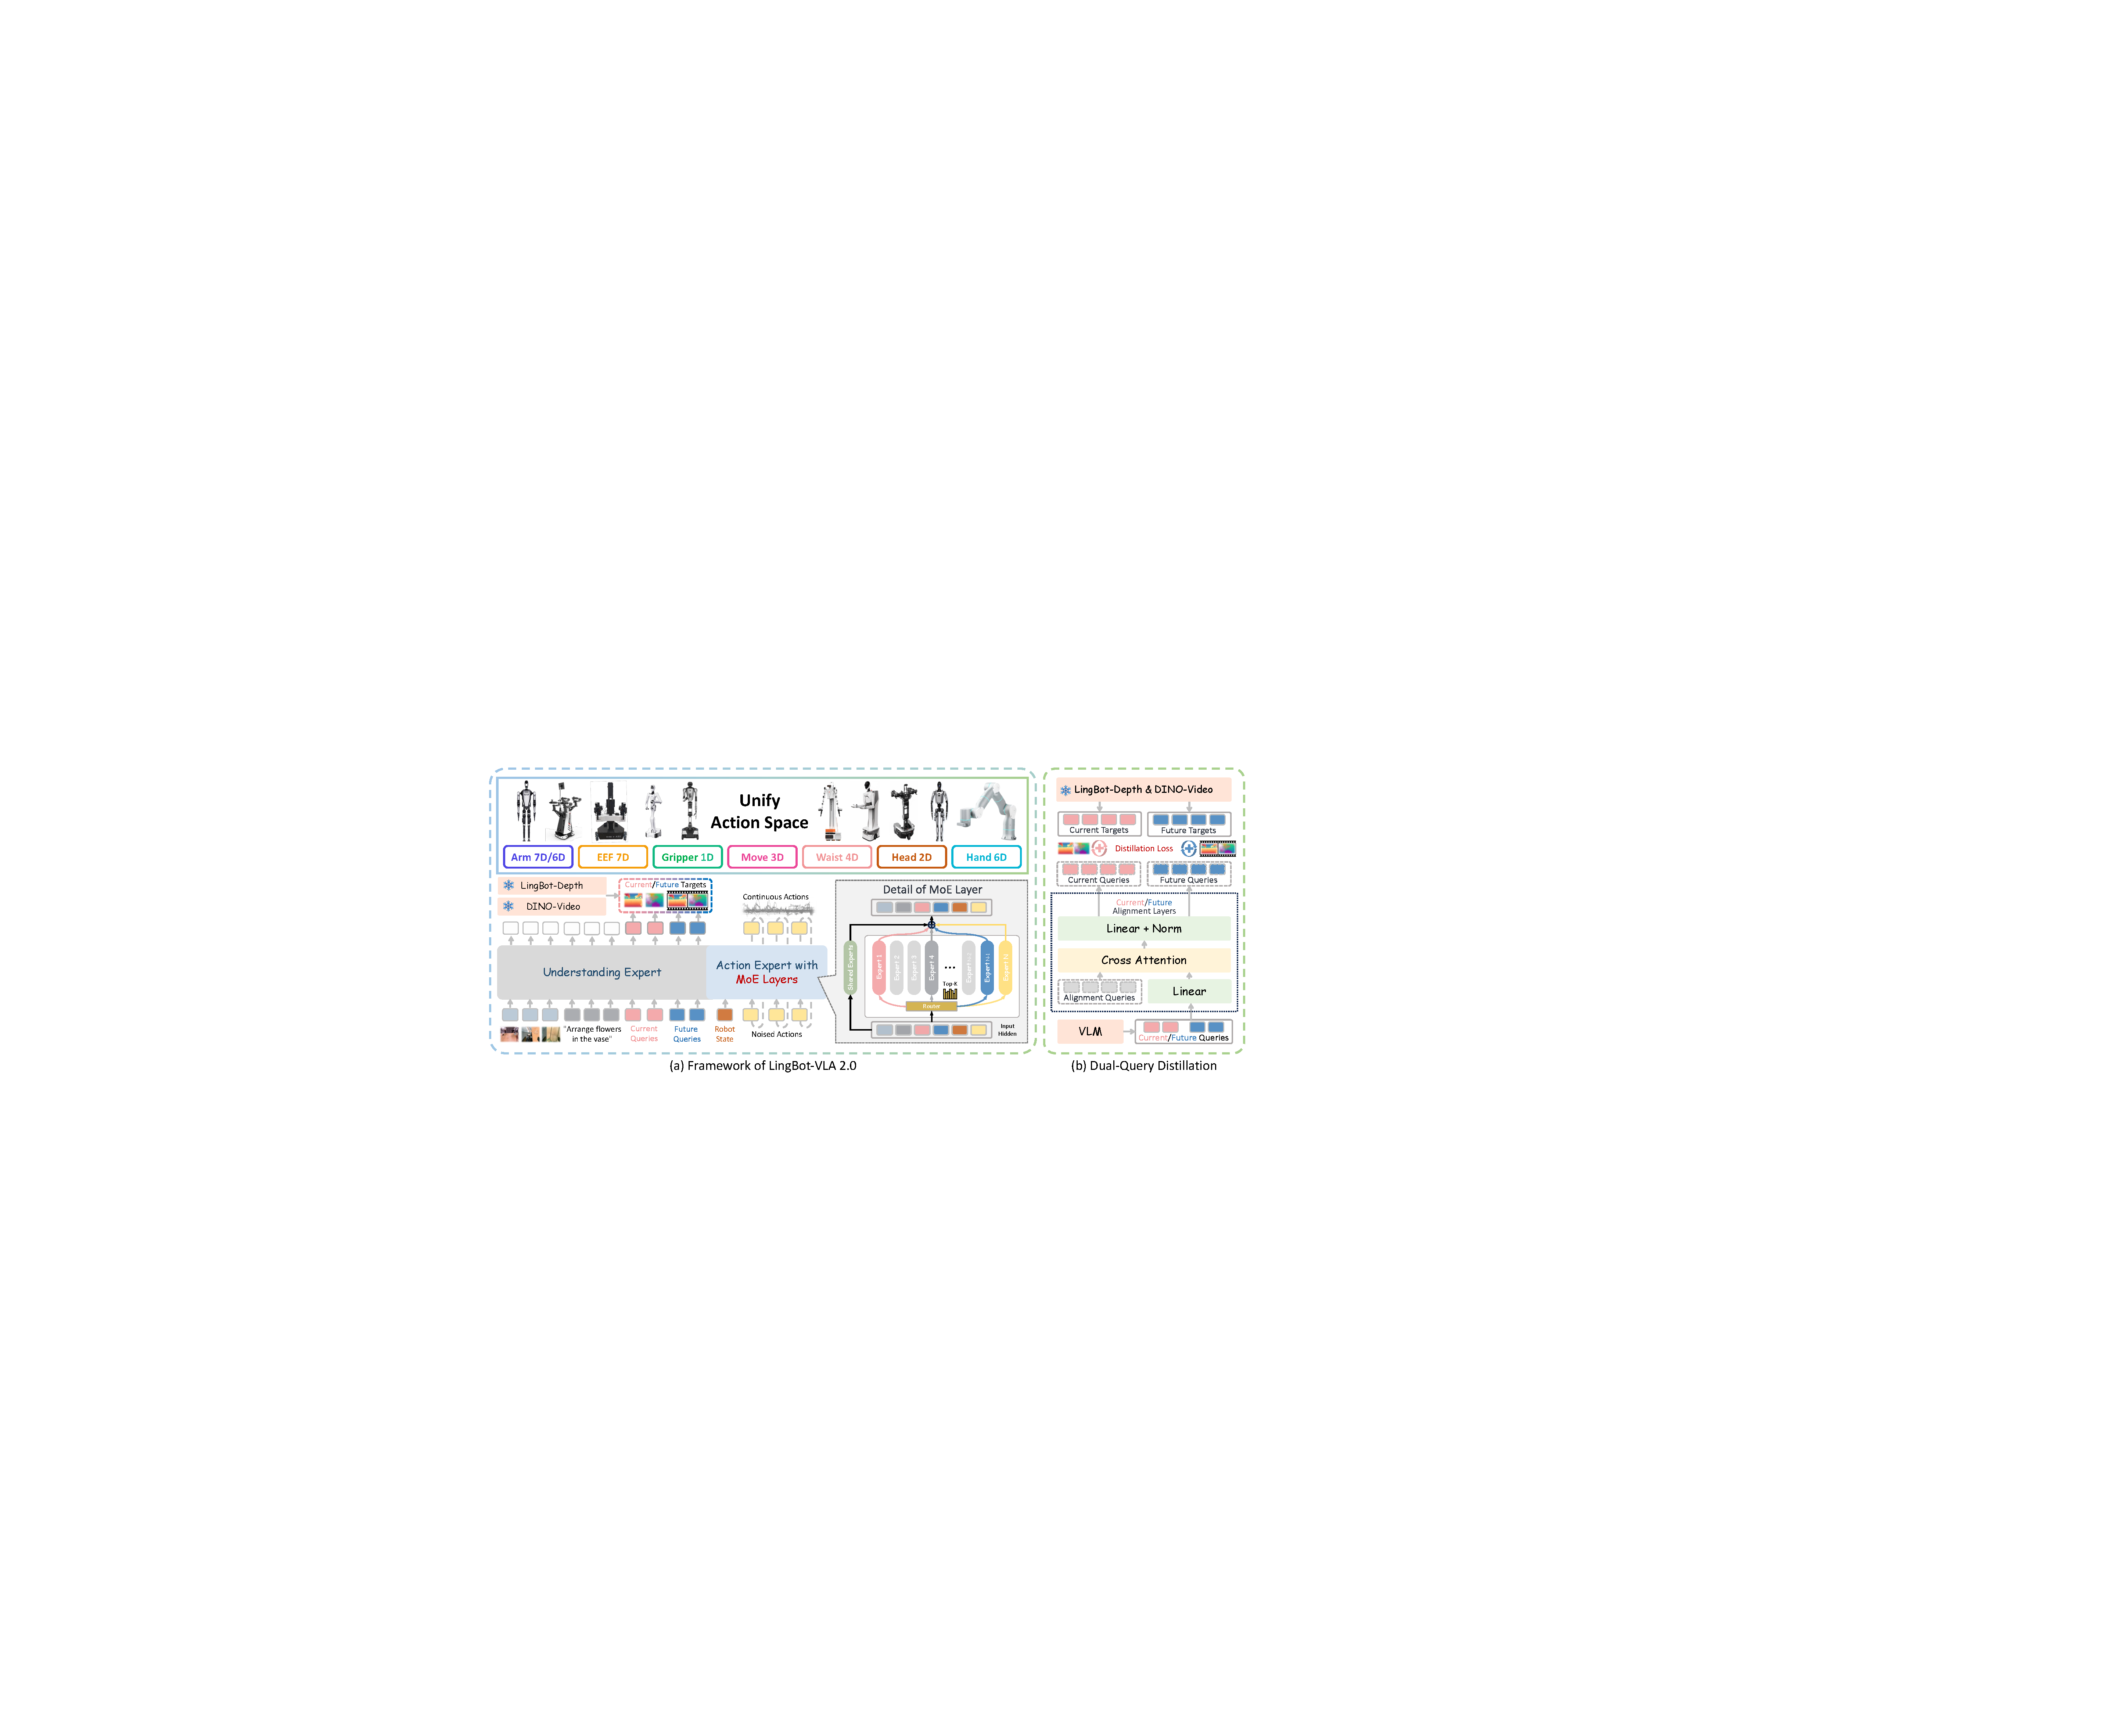
\includegraphics[width=\linewidth]{figures/framework.pdf}
\caption{\textbf{Overview of \method}. We revamp the data processing pipeline and curate 60,000 hours of pretraining data, including 50,000 hours of robot trajectories across 20 robot configurations and 10,000 hours of egocentric human videos. Moreover, our model supports degrees of freedom for the head, waist, mobile base, and dexterous hands, enabling robots to handle more complex real-world tasks. We formulate future prediction as a proxy task, leveraging a video representation model for semantic priors and a depth estimation model for geometric cues.}
\label{fig:teaser}
\end{figure}


\section{Introduction}\label{sec:intro}

Vision-language-action (VLA) models~\cite{pi_0,pi_0d5,gr00tN1,openvla} have recently emerged as a promising paradigm for building generalist robot policies. 
A key advantage of this paradigm is that pretrained vision-language models provide rich multimodal alignment and semantic representations, enabling VLA models to better understand complex scenes and generalize across diverse tasks.
Beyond such model-level priors, recent advances~\cite{pi_0d5,generalist2026gen1} further show that scaling up robot data in both quantity and diversity can substantially improve the capability of VLA systems.
Together, these developments have established VLA as a compelling foundation for robot learning.

However, despite this rapid progress, a substantial gap remains between laboratory benchmarks and real-world deployment. 
In practice, robots are expected to operate under broader embodiment diversity, richer action spaces, and more dynamic environments than those considered in many existing VLA settings. 
First, generalization in practice is not only about transferring across tasks, but also about handling heterogeneous robot configurations and data sources. 
Another point is that many real-world platforms involve substantially more degrees of freedom than standard dual-arm manipulation setups, including head movement, waist, mobile-base control, and dexterous hands. 
Subsequently, real-world execution often requires anticipating future scene evolution and action consequences, rather than reacting only to current observations. 
These challenges collectively limit the practical utility of current VLA foundation models.

A growing body of work has started to address these issues from different perspectives. Some approaches~\cite{beingH05,generalist2026gen1,lingbotvla} scale robot pretraining data to improve cross-task and cross-embodiment robustness.
Others incorporate embodiment-aware architectural designs~\cite{g0_5} to better handle heterogeneous robots. 
Another line of research augments VLA models with latent action model~\cite{dexWorldModel,lda1b} to improve decision making in dynamic environments. Meanwhile, recent system-oriented efforts have emphasized that practical VLA deployment depends not only on model scale, but also on data quality, action coverage, and training objectives that better align pretraining with downstream execution. These trends indicate that improving VLA models in practice requires a coordinated treatment of data, embodiment, and predictive capability.

In this work, we build on this perspective and present \method, an improved version of \methodold aimed at bridging foundation-level VLA capabilities with practical robotic deployment. Rather than focusing on a single improvement, \method advances the system along three functional domains that we find particularly critical for real-world deployment. First, to improve \textbf{\textit{generalization}} across tasks and embodiments, we redesign the data processing pipeline and curate a large-scale pretraining corpus of around 60,000 hours, including 50,000 hours of robot trajectories spanning \robotnum robot configurations and 10,000 hours of egocentric human videos. This design aims to provide broader coverage over both embodiment patterns and interaction scenarios. Second, to support a wider range of practical robots, we extend the model to an \textbf{\textit{expanded action space}} beyond standard dual-arm platforms, enabling control over the head, waist, mobile base, and dexterous hands. This expanded control interface allows the system to address more complex tasks that require coordinated whole-body interaction. Third, to improve temporal reasoning in dynamic environments, as shown in~\cref{fig:teaser}, we introduce \textbf{\textit{predictive dynamics modeling}} as a proxy objective. Concretely, we formulate future prediction using a video representation model to provide semantic priors and a depth estimation model to provide geometric cues, encouraging the VLA model to reason about future scene evolution and action consequences. Our central hypothesis is that practical VLA systems should not only scale in model and data size, but also become better aligned with the demands of real-world robotics: broader embodiment support, richer controllable action spaces, and stronger predictive understanding of dynamic scenes. Under this view, \method is intended as a step from foundation-level capability toward application-oriented usability.

We evaluate \method in a generalist setting on nine tasks from the GM-100 dual-arm manipulation benchmark~\cite{gm100}, as well as on two long-horizon mobile manipulation tasks. The results show that the proposed modifications consistently improve practical capability, validating the importance of jointly enhancing generalization, action-space coverage, and predictive dynamics modeling. Overall, our work highlights a pragmatic direction for advancing VLA foundation models from laboratory success toward real-world applicability.
